\documentclass[a4]{beamer}
\usepackage{amssymb}
\usepackage{graphicx}
\usepackage{subfigure}
\usepackage{newlfont}
\usepackage{amsmath,amsthm,amsfonts}
%\usepackage{beamerthemesplit}
\usepackage{pgf,pgfarrows,pgfnodes,pgfautomata,pgfheaps,pgfshade}
\usepackage{mathptmx}  % Font Family
\usepackage{helvet}   % Font Family
\usepackage{color}

\mode<presentation> {
 \usetheme{Default} % was
 \useinnertheme{rounded}
 \useoutertheme{infolines}
 \usefonttheme{serif}
 %\usecolortheme{wolverine}
% \usecolortheme{rose}
\usefonttheme{structurebold}
}

\setbeamercovered{dynamic}

\title[MA4413]{Statistics for Computing \\ {\normalsize MA4413 Lecture 10B}}
\author[Kevin O'Brien]{Kevin O'Brien \\ {\scriptsize Kevin.obrien@ul.ie}}
\date{Autumn Semester 2013}
\institute[Maths \& Stats]{Dept. of Mathematics \& Statistics, \\ University \textit{of} Limerick}

\renewcommand{\arraystretch}{1.5}


\begin{document}


\begin{frame}
\titlepage
\end{frame}

%---------%
\begin{frame}
\frametitle{Using \texttt{R} for Inference Procedures}
\begin{itemize}
\item[1] Review of the Paired t-test.
\item[2] Paired t-test using \texttt{R}
%\item[3] Two Sample Test for Proportions
\item[3] Test for the equality of variances for two samples
\item[4] Shapiro-Wilk Test for Normality
\item[5] Graphical procedures for assessing normality
\item[6] Grubb's Procedure for Determinin an Outlier
\end{itemize}
\end{frame}
%---------%
\begin{frame}
\frametitle{p-values using \texttt{R}}
\begin{itemize}
\item In every inference procedure performed using \texttt{R}, a p-value is presented to the screen for the user to interpret.

\item If the p-value is larger than a specified threshold $\alpha/k$ then the appropriate conclusion is a
failure to reject the null hypothesis.

\item Conversely, if the p-value is less than threshold, the appropriate conclusion is to reject the null hypothesis.

\item In this module, we will use a significance level$\alpha=0.05$ and almost always the procedures will be two tailed ($k=2$). Therefore the threshold $\alpha/k$ will be $0.025$.
\end{itemize}
\end{frame}

%---------%
\begin{frame}
\frametitle{Using Confidence Limits}
\begin{itemize}
\item Alternatively, we can use the confidence interval to make a decision on whether or not we should reject or fail to reject the null hypothesis.
\item If the null value is within the range of the confidence limits, we fail to reject the null hypothesis.
\item If the null value is outside the range of the confidence limits, we reject the null hypothesis.
\item Occasionally a conclusion based on this approach may differ from a conclusion based on the p-value. In such a case, remark upon this discrepancy.
\end{itemize}
\end{frame}
%------------------------------------------%

\begin{frame}
\frametitle{The paired t-test (a)}

\begin{itemize}
\item Previously we have seen the paired t-test. It is used to determine whether or
not there is a significant difference between paired measurements. Equivalently whether or not
the case-wise differences are zero.
\item The mean and standard deviation of the case-wise differences are used to determine the test statistic.
\item Under the null hypothesis, the expected value of the case-wise differences is zero (i.e $H_0 : \mu_d = 0$).
\item The test statistic is computed as
\[ TS = \frac{\bar{d} - \mu_d}{\frac{s_d}{\sqrt{n}}} \]
\end{itemize}
\end{frame}


%------------------------------------------%
\begin{frame}[fragile]
\frametitle{The Paired t-test (b)}
\begin{itemize}
\item The calculation is dependent on the case-wise differences.
\item Here the case-wise differences between paired measurements (e.g. ``before" and ``after").
\item Under the null hypothesis, the mean of case-wise differences is zero.
\item As a quick example, the mean, standard deviation and sample size are presented in the next slide.
\end{itemize}
\end{frame}

%------------------------------------------%
\begin{frame}[fragile]
\frametitle{The paired t-test (c)}
\begin{itemize}
\item Observed Mean of Case-wise differences $\bar{d}$ = 8.21,
\item Expected Mean of Case-wise differences under $H_0$ : $\mu_d = 0$,
\item Standard Deviation of Case-wise differences $S_d$ = 7.90,
\item Sample Size $n=14$.
\end{itemize}

\[ TS = \frac{\bar{d} - \mu_d}{\frac{s_d}{\sqrt{n}}} = \frac{8.21 - 0}{\frac{7.90}{\sqrt{14}}} = 3.881 \]
\end{frame}
%------------------------------------------%
\begin{frame}[fragile]
\frametitle{The paired t-test (e)}

\begin{itemize}
\item Procedure is two-tailed, and you can assume a significance level of 5\%.
\item It is also a small sample procedure (n=14, hence df = 13).
\item The Critical value is determined from statistical tables (2.1603).
\item Decision Rule: Reject Null Hypothesis ($|TS|>CV$). Significant difference in measurements before and after.
\end{itemize}

\end{frame}
%------------------------------------------%
\begin{frame}[fragile]
\frametitle{The paired t-test (f)}
Alternative Approach : using p-values.
\begin{itemize}
\item The p-values are determined from computer code. (We will use a software called \texttt{R}. Other types of software inlcude \texttt{SAS} and \texttt{SPSS}.)
\item The null and alternative are as before.
\item The computer software automatically generates the appropriate test statistic, and hence the corresponding p-value.
\item The user then interprets the p-values. If p-value is small, reject the null hypothesis. If the p-value is large, the appropriate conclusion is a failure to reject $H_0$.
\item The threshold for being considered small is less than $\alpha/k$, (usually 0.0250). (This is a very arbitrary choice of threshold, suitable for some subject areas, not for others)
\end{itemize}
\end{frame}
%------------------------------------------%
\begin{frame}[fragile]
\frametitle{The paired t-test (g)}
Implementing the paired t-test using \texttt{R} for the example previously discussed.
\begin{verbatim}
> t.test(Before,After,paired=TRUE)

        Paired t-test

data:  Before and After
t = 3.8881, df = 13, p-value = 0.001868
alternative hypothesis: true difference in means is not 0
95 percent confidence interval:
  3.650075 12.778496
sample estimates:
mean of the differences
               8.214286

\end{verbatim}
\end{frame}

%-------------------------------------------------%
\begin{frame}[fragile]
\frametitle{The paired t-test (h)}
\begin{itemize}
\item The p-value ($0.001868$) is less than the threshold is less than the threshold $0.0250$.
\item We reject the null hypothesis (mean of case-wise differences being zero, i.e. expect no difference between ``before" and ``after").
\item We conclude that there is a difference between `before' and `after'.
\item That is to say, we can expected a difference between two paired measurements.
\end{itemize}
\end{frame}
%-------------------------------------------------%
\begin{frame}[fragile]
\frametitle{The paired t-test (i)}
\begin{itemize}
\item We could also consider the confidence interval. We are $95\%$ confident that the expected value of the case-wise difference is at least 3.65.
\item Here the null value (i.e. 0) is not within the range of the confidence limits.
\item Therefore we reject the null hypothesis.
\end{itemize}
\begin{verbatim}
> t.test(Before,After,paired=TRUE)
...
...
95 percent confidence interval:
  3.650075 12.778496
...
\end{verbatim}
\end{frame}



%----------------------------------------%

\begin{frame}

\frametitle{Test for Equality of Variance (a)}
\begin{itemize}
\item In this procedure, we determine whether or not two populations have the same variance.
\item The assumption of equal variance of two populations underpins several inference procedures. This assumption is tested by comparing the variance of samples taken from both populations.
\item We will not get into too much detail about that, but concentrate on how to assess equality of variance.
\item The null and alternative hypotheses are as follows:
\[ H_0: \sigma^2_1 = \sigma^2_2 \]
\[ H_1: \sigma^2_1 \neq \sigma^2_2 \]
\end{itemize}

\end{frame}
%----------------------------------------%
\begin{frame}
\frametitle{Test for Equality of Variance (b)}
\begin{itemize}
\item When using \texttt{R} it would be convenient to consider the null and alternative in terms of variance ratios.
\item Two data sets have equal variance if the variance ratio is 1.
\end{itemize}

\[ H_0: \sigma^2_1 / \sigma^2_2 = 1 \]
\[ H_1: \sigma^2_1 / \sigma^2_2 \neq 1 \]
\end{frame}
%----------------------------------------%
% - x=c(14,13,16,20,12,18,11,09,13,11)
% - y=c(15,13,18,20,10,17,23,11,10)
%----------------------------------------%
\begin{frame}[fragile]
\frametitle{Test for Equality of Variance(c)}
You would be required to compute the test statistic for this procedure.
The test statistic is the ratio of the variances for both data sets.
\[ TS = \frac{s^2_x}{s^2_y} \]
The standard deviations would be provided in the \texttt{R} code. \begin{itemize}
\item Sample standard deviation for data set $x$ = 3.40
\item Sample standard deviation for data set $y$ = 4.63
\end{itemize}
To compute the test statistic.
\[ TS = \frac{3.40^2}{4.63^2} = \frac{11.56}{21.43} = 0.5394 \]

\end{frame}
%----------------------------------------%
\begin{frame}[fragile]
\frametitle{Variance Test (d)}
\begin{verbatim}
> var.test(x,y)

        F test to compare two variances

data:  x and y
F = 0.5394, num df = 9, denom df = 8, p-value = 0.3764
alternative hypothesis: 
 true ratio of variances is not equal to 1
95 percent confidence interval:
 0.1237892 2.2125056
sample estimates:
ratio of variances
         0.5393782
\end{verbatim}

\end{frame}
%----------------------------------------%

\begin{frame}
\frametitle{Variance Test (e)}
\begin{itemize}
\item The p-value is 0.3764 (top right), above the threshold level of 0.0250.
\item We fail to reject the null hypothesis.
\item We can assume that there is no significant difference in sample variances. Therefore we can assume that both populations have equal variance.
\item Additionally the $95\%$ confidence interval (0.1237, 2.2125) contains the null values i.e. 1.
\end{itemize}
\end{frame}


%-------------------------------------------------%


\begin{frame}
\frametitle{Shapiro-Wilk Test(a)}


\begin{itemize}
\item We will often be required to determine whether or not a data set is normally distributed.
\item Again, this assumption underpins many statistical models.
\item The null hypothesis is that the data set is normally distributed.
\item The alternative hypothesis is that the data set is not normally distributed.
\item One procedure for testing these hypotheses is the Shapiro-Wilk test, implemented in \texttt{R} using the command \texttt{shapiro.test()}.
\item (Remark: You will not be required to compute the test statistic for this test.)
\end{itemize}
\end{frame}
%----------------------------------------%
\begin{frame}[fragile]
\frametitle{Shapiro Wilk Test(b)}
For the data set used previously; $x$ and $y$, we use the Shapiro-Wilk test to determine that both data sets are normally distributed.
\begin{verbatim}

> shapiro.test(x)

        Shapiro-Wilk normality test

data:  x
W = 0.9474, p-value = 0.6378

> shapiro.test(y)

        Shapiro-Wilk normality test

data:  y
W = 0.9347, p-value = 0.5273
\end{verbatim}

\end{frame}


%-------------------------------------------------%
\begin{frame}[fragile]
\frametitle{Graphical Procedures for assessing Normality}

\begin{itemize}
\item The normal probability (Q-Q) plot is a very useful tool for determining whether or not a data set is normally distributed.
\item Interpretation is simple. If the points follow the trendline (provided by the second line of \texttt{R} code \texttt{qqline}).
\item One should expect minor deviations. Numerous major deviations would lead the analyst to conclude that the data set is not normally distributed.
\item The Q-Q plot is best used in conjunction with a formal procedure such as the Shapiro-Wilk test.
\end{itemize}

\begin{verbatim}
>qqnorm(CWdiff)
>qqline(CWdiff)
\end{verbatim}

\end{frame}

%-------------------------------------------------%

\begin{frame}
\frametitle{Graphical Procedures for Assessing Normality}

\begin{center}
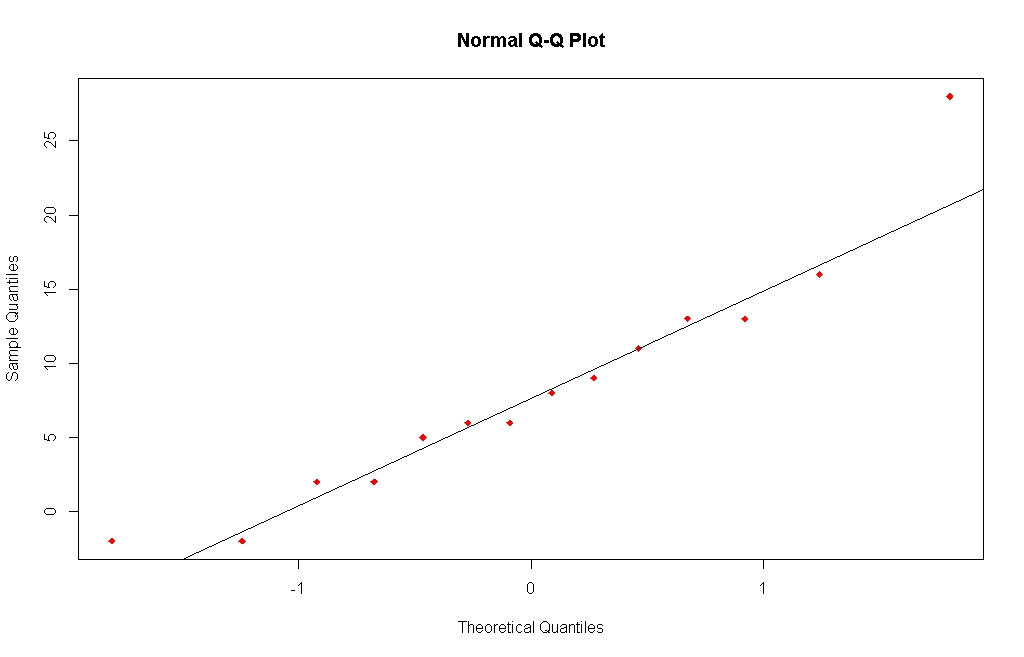
\includegraphics[scale=0.32]{10AQQplot}
\end{center}
\end{frame}
%----------------------------------------------------------%
\begin{frame}[fragile]
\frametitle{Grubbs Test for Determining an Outlier}

The Grubbs test is used to determine if there are any outliers in a data set.\\ \bigskip
There is no agreed formal definition for an outlier. The definition of outlier used for this procedure is a value that unusually distance from the rest of the values ( For the sake of clarity , we shall call this type of outlier a \textbf{Grubbs Outlier}). Consider the following data set: is the lowest value 4.01 an outlier?
\begin{verbatim}
6.98 8.49 7.97 6.64
8.80 8.48 5.94 6.94
6.89 7.47 7.32 4.01
\end{verbatim}

Under the null hypothesis, there are no outliers present in the data set. 
We reject this hypothesis if the p-value is sufficiently small.
\end{frame}

%-------------------------------------------------%
\begin{frame}[fragile]
\frametitle{Grubbs Test for Determining an Outlier}
\begin{verbatim}
> grubbs.test(x, two.sided=T)
Grubbs test for one outlier
data: x
G = 2.4093, U = 0.4243, p-value = 0.05069
alternative hypothesis: lowest value 4.01 is an outlier
\end{verbatim}
We conclude that while small by comparison to the other values, the lowest value 4.01 is not an outlier.
\end{frame}

\end{document}


%-------------------------------------------------%
%-------------------------------------------------%
\begin{frame}[fragile]
\frametitle{Single Sample Proportion Test (a)}

\begin{itemize}
\item In this procedure, we determine whether or not we are are justified in assuming that the population proportion takes a certain value.
\item For example, suppose we believed that the population proportion of students with iphones or androids was $80\%$.
\item We would write the null and alternative accordingly.
\[H_0 : \pi = 80\% \]
\[H_1 : \pi \neq 80\% \]
\item The  appropriate \texttt{R} command is \texttt{prop.test(x,n,p)}
\item $x$ is the number of successes, $n$ is the sample size and $p$ is the population proportion assumed under the null hypothesis.
\item Suppose we survey 65 students, with 50 replying that they had an iphone or android.
\end{itemize}

\end{frame}
%-------------------------------------------------%

\begin{frame}[fragile]
\frametitle{Single Sample Proportion Test (b)}

\begin{verbatim}
> prop.test(50,65,0.80)

        1-sample proportions test

data:  50 out of 65, null probability 0.8
X-squared = 0.2163, df = 1, p-value = 0.6418
alternative hypothesis: true p is not equal to 0.8
95 percent confidence interval:
 0.6452269 0.8610191
sample estimates:
        p
0.7692308
\end{verbatim}

\end{frame}

\begin{frame}[fragile]
\frametitle{Single Sample Proportion Test (c)}

\begin{itemize}
\item The p-value is above the threshold. Therefore we fail to reject the null hypothesis that the population proportion ($\pi$) is $80\%$.

\item The observed proportion is a very straightforward calculation:

\[ \hat{p} = \frac{50}{65} = 0.76923= 76.92\%\]
\item Nonetheless, you would be required to show how it was calculated.
\end{itemize}

\end{frame}

%-------------------------------------------------%
\begin{frame}[fragile]
\frametitle{Test of Equality for Two Sample Proportions (a)}
The null hypothesis is that two populations have the same proportions for a particular characteristic.
\[H_0 : \pi_1 = \pi_2 \]
\[H_1 : \pi_1 \neq \pi_2 \]
\begin{itemize}
\item The command is \texttt{prop.test(c(x1,x2),c(n1,n2))}
\item $x1$ and $x2$ are the number of successes from both samples.
\item $n2$ and $n2$ are the sample sizes for both groups.
\item The difference in population proportions assumed under the null hypothesis is zero.
\item (It is possible to specify a different null value, but we will not consider this in this module.)
\end{itemize}
\end{frame}

%-------------------------------------------------%
\begin{frame}
\frametitle{Test of Equality for Two Sample Proportions (b)}
\begin{itemize}
\item Consider a study where the proportion of Irish students who owned mobile devices, such as iphones and androids was compared to the corresponding proportion of French student.
\item As before, $65$ Irish students were interviewed, with $50$ replying that they owned mobile devices.
\item $90$ french students were interview, with 60 responding that they owned mobile devices.
\item The test of equality of proportions is implemented on the next slide.
\end{itemize}
\end{frame}

%-------------------------------------------------%


\begin{frame}[fragile]
\frametitle{Test of Equality for Two Sample Proportions (c)}
Based on the p-value, we fail to reject the null hypothesis. There is not enough evidence to assume a difference in proportions. Also the expected difference assumed under the null hypothesis, i.e. 0, is contained in the confidence interval.
\begin{verbatim}
> prop.test(c(50,60),c(65,90))

        2-sample test for equality of proportions

data:  c(50, 60) out of c(65, 90)
X-squared = 1.4613, df = 1, p-value = 0.2267
alternative hypothesis: two.sided
95 percent confidence interval:
 -0.05202058  0.25714878
sample estimates:
   prop 1    prop 2
0.7692308 0.6666667
\end{verbatim}
\end{frame}
\begin{frame}[fragile]
\frametitle{Test of Equality for Two Sample Proportions (d)}
\begin{itemize}
\item You would be required to compute the differences in observed proportions.
\item Additionally you will given the \texttt{R} code for one sample procedures. This may or may not be relevant for answering the question.
\end{itemize}
\begin{verbatim}
> prop.test(60,90,0.80)
...
...
X-squared = 9.184, df = 1, p-value = 0.002441
alternative hypothesis: true p is not equal to 0.8
95 percent confidence interval:
 0.5585219 0.7604058
sample estimates:
        p
0.6666667
\end{verbatim}

\end{frame}
%-------------------------------------------------%

Kolmogorov Smirnov Tests
Non-parametric procedures
Compute the test statistic
Same distribution
